\section{Impact of initial mutual inclination}\label{sec:inclination}


In this section, I investigate the importance of the initial mutual inclination on the evolution of the system. I present a comparison between simulations  1, 2 \& 3 listed in \cref{tab:simulations_settings}, which correspond to different initial inclination of the outer orbit relative to the inner orbit


\subsection{Outer orbit}

In \cref{fig:incliantion_tertiary_mass}, I present the evolution of the tertiary's mass for different initial mutual inclination. First, I would like to point out that the case of $i_{mut} = 69^{\circ}$ is not directly comparable to the other two cases. In order to place the tertiary initially at a higher inclination, the positions of all particles in the 3D model are corrected for the appropriate angle. Then the center of mass of the tertiary corresponds to the center of mass of all these particles. In this case, numerical rounding resulted into a shorter initial separation between the giant and the center of mass of the inner binary, see \cref{fig:inclination_outer_semimajor_axis}. More specifically, the tertiary was placed $\approx 0.01$ au ($\approx 2.15 R_{\odot}$) closer. This may seem as a small difference, but it has a significant impact on the mass loss rate. The smaller initial separation corresponds to higher fractional radius excess of the tertiary and considering \cref{eq:mass_loss_rate_anal}, the mass loss rate is highly overestimated in comparison with the other two models, see also \cref{fig:incliantion_tertiary_mass}.  As a result, the rate of decay of the outer orbit for the $i_{mut} = 69^{\circ}$ case is also overestimated compared to the other two models.
\begin{figure}[!htb]
    \centering
    \begin{subfigure}{.5\textwidth}
    \centering
    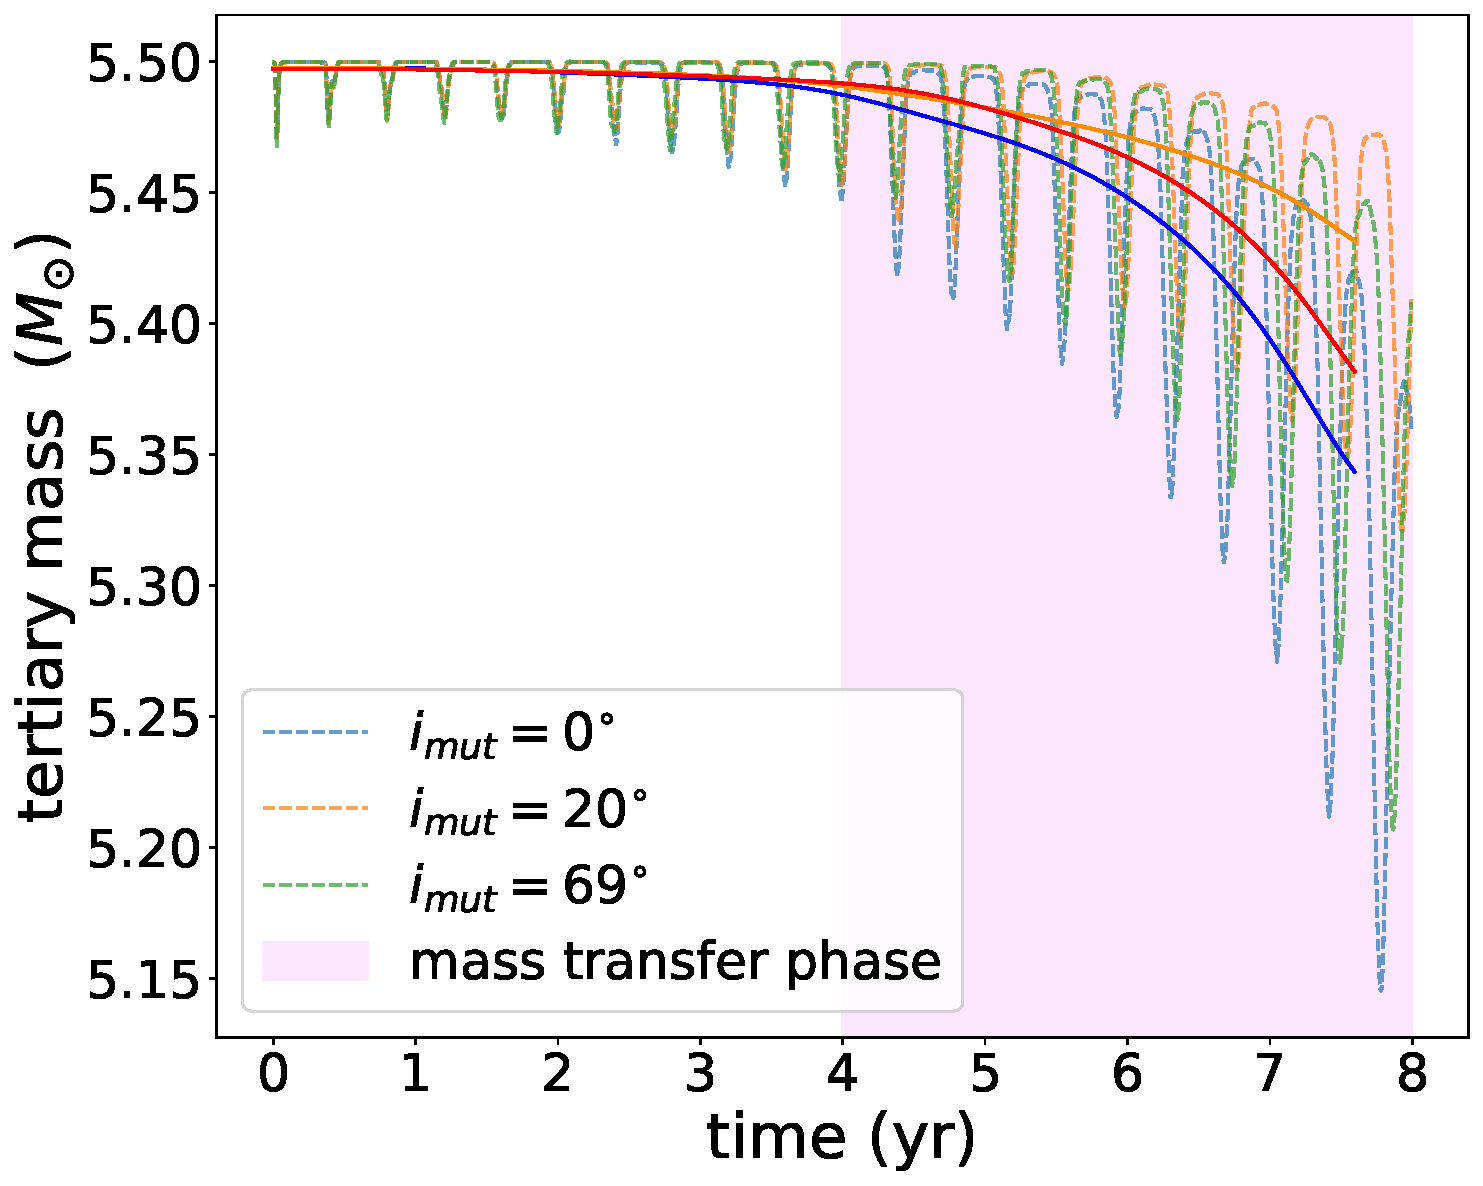
\includegraphics[width=0.9\textwidth]{Thesis/graphs/inclination_case/inclination_mass_loss.pdf}
    \end{subfigure}%
    \begin{subfigure}{.5\textwidth}
    \centering
    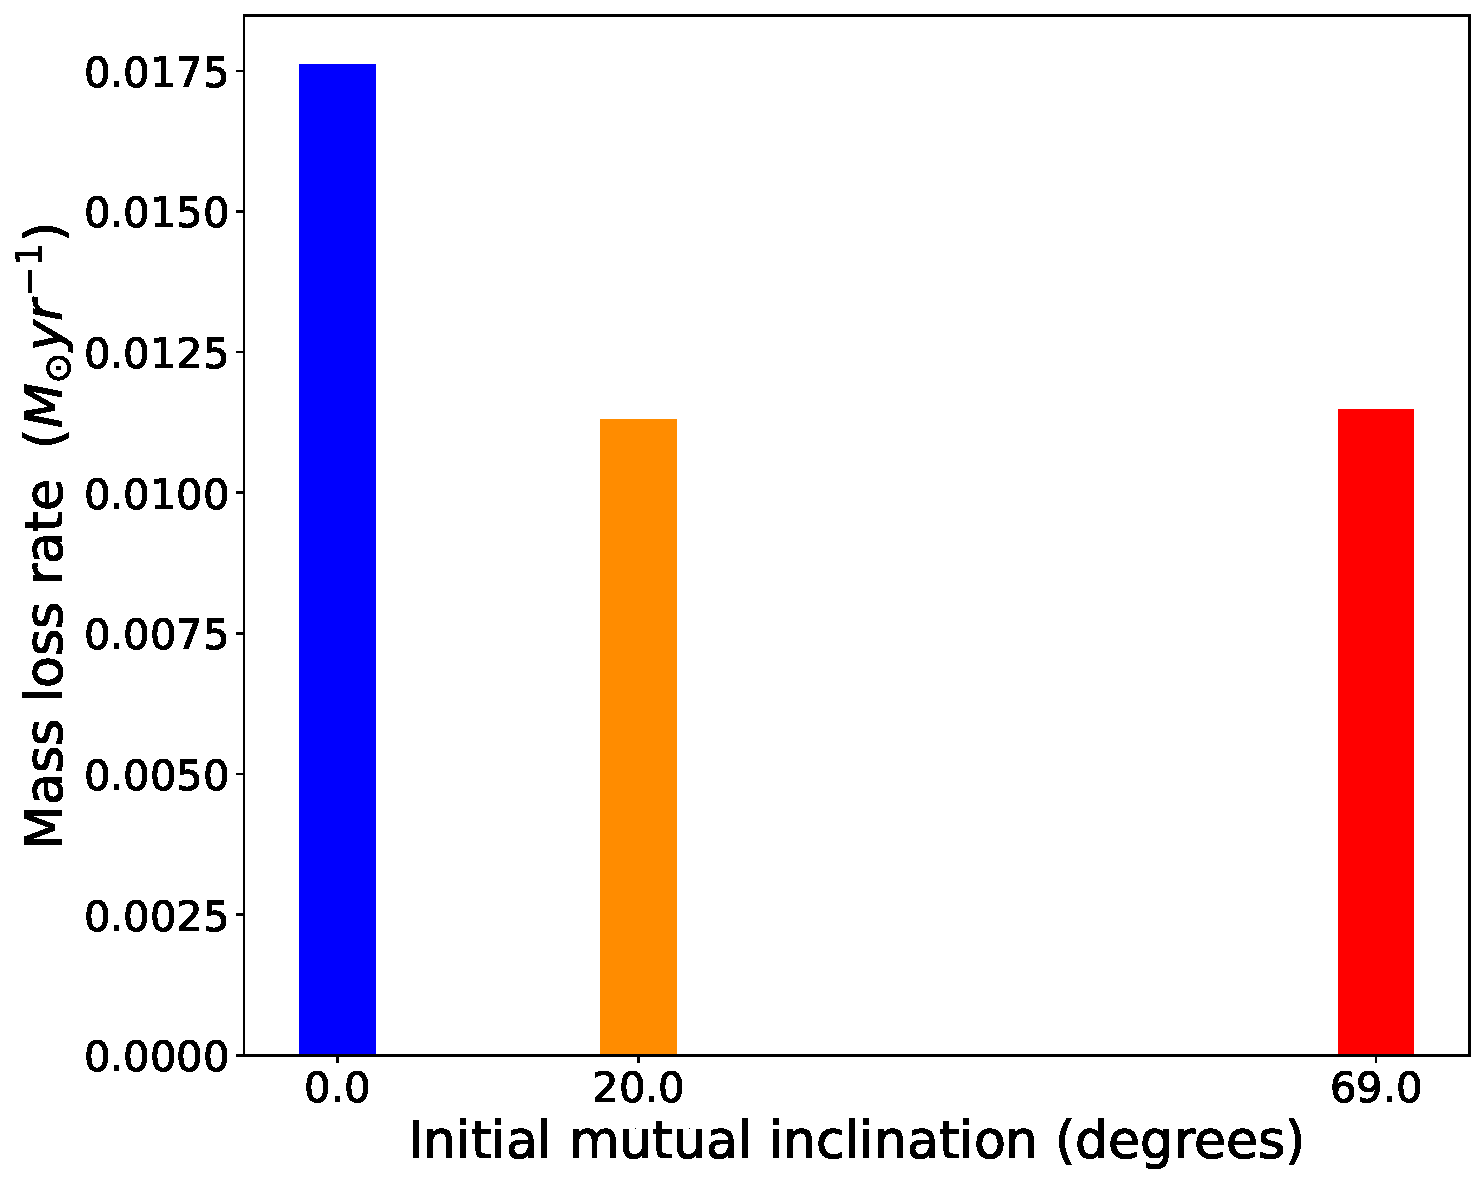
\includegraphics[width=0.9\textwidth]{Thesis/graphs/inclination_case/incliantion_giant_mass_loss_rate.pdf}
    \end{subfigure}
    \caption{ The evolution of the tertiary's mass (left) for of the outer orbit for different initial inclination of the outer orbit relative to the inner orbit. The simulated data is shown in dashed lines. The continues lines are smooth representations of the simulated data in their respective colors. The last three orbits are not included in the smoothed version, because the lack of data above $8$ yr will erroneously flatten the slopes. The mean mass loss rates computed using central differentiation on the simulated data (right).}
    \label{fig:incliantion_tertiary_mass}
\end{figure}

Keeping in mind that the mass loss rate for the case of $i_{mut} = 69^{\circ}$ is overestimated, I speculate that there is a trend: lower initial mutual inclination results to higher mass loss rate for the tertiary. This is not a surprise, as each of the inner binary stars can approach the giant closer for orbits that are nearly on the same plane. Additionally, the mass loss rate derived using central differentiation on the simulated data are in good agreement with the analytical ones calculated using \cref{eq:mass_loss_rate_anal}.
\begin{figure}[H]
    \centering
    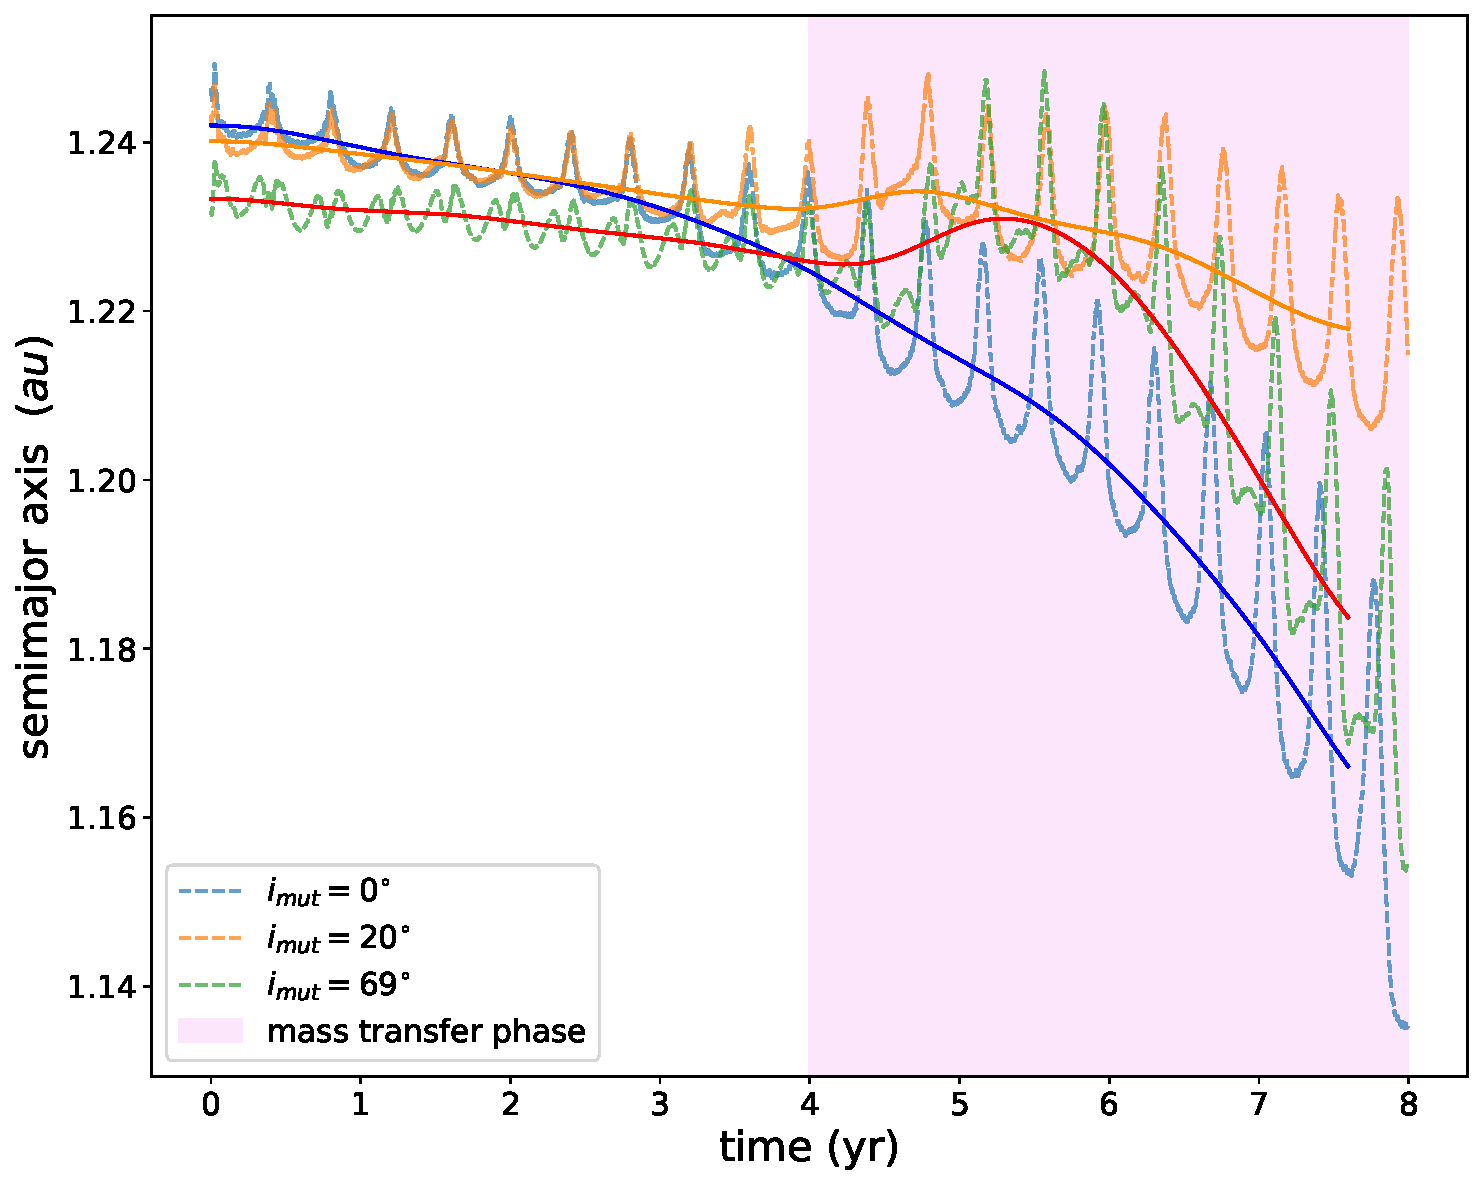
\includegraphics[width=0.85\textwidth]{Thesis/graphs/inclination_case/inclination_outer_semimajor_axis.pdf}
    \caption{Evolution of the semi-major axis of the outer orbit for different initial inclination of the outer orbit relative to the inner orbit. The simulated data is shown in dashed lines. The continues lines are smooth representations of the simulated data in their respective colors. The last three orbits are not included in the smoothed version, because the lack of data above $8$ yr will erroneously flatten the slopes.}
    \label{fig:inclination_outer_semimajor_axis}
\end{figure}
In \cref{fig:inclination_outer_semimajor_axis}, I display the evolution of the semi-major axis for different initial mutual inclinations. Considering only the $i_{mut} = 0^{\circ} \; \&  \; 20^{\circ}$ cases, the outer orbit decays faster for lower initial mutual inclination, because more mass is transferred towards the inner binary carrying away orbital angular momentum. 

In \cref{fig:inclination_outer_ecc},  the evolution of the eccentricity for different initial mutual inclinations is illustrated. Furthermore, in \cref{fig:mutual_inclination}, I present the evolution of the mutual inclination between the inner and the outer orbit for initial $i_{mut} = 20^{\circ}, 69^{\circ}$. The $i_{mut} = 0^{\circ}$ case is already displayed in \cref{fig:accretion_inc}.  Tidal interactions, as predicted, tend to circularize the outer orbit and also bring it towards coplanarity with the inner orbit.
\begin{figure}[H]
    \centering
    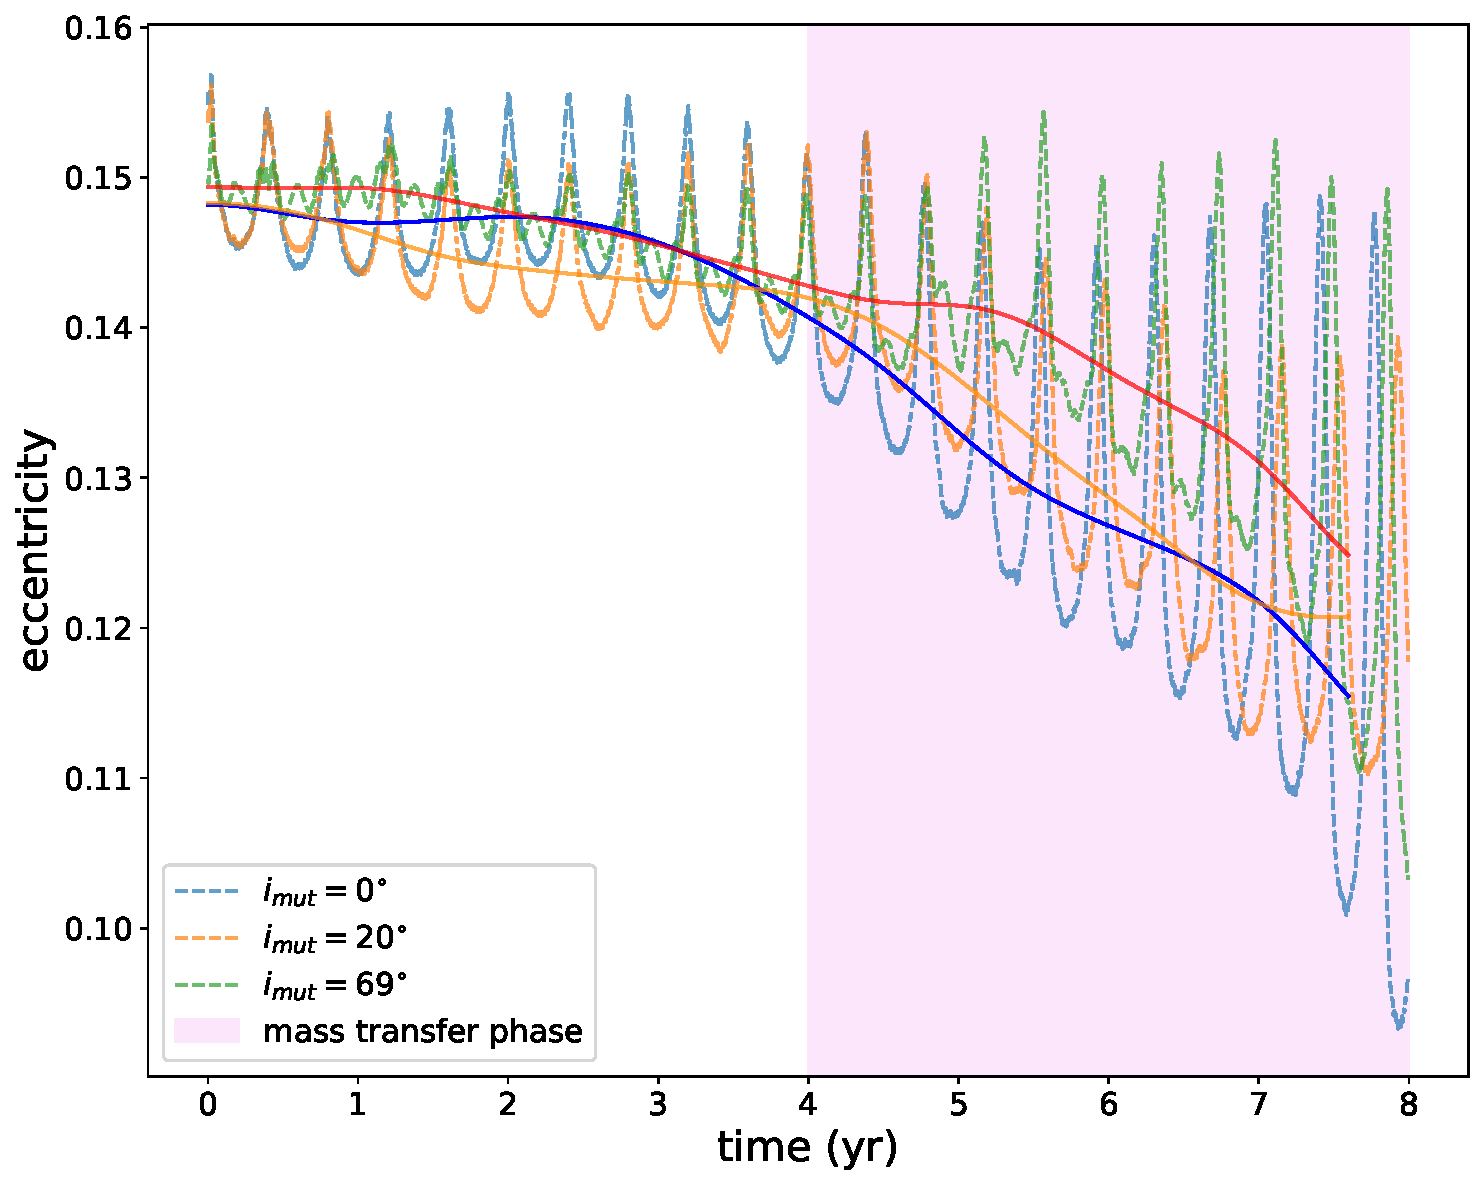
\includegraphics[width=0.9\textwidth]{Thesis/graphs/inclination_case/inclination_outer_ecc.pdf}
    \caption{Evolution of the eccentricity of the outer orbit for different initial inclination of the outer orbit relative to the inner orbit. The simulated data is shown in dashed lines. The continues lines are smooth representations of the simulated data in their respective colors. The last three orbits are not included in the smoothed version, because the lack of data above $8$ yr will erroneously flatten the slopes.}
    \label{fig:inclination_outer_ecc}
\end{figure}
As the giant, approaches the inner binary, the outer orbit tends to be circular, see \cref{fig:inclination_outer_ecc}. The interesting point though comes from a comparison between $i_{mut} = 20^{\circ} \& 69^{\circ}$. Despite the fact that for $i_{mut} = 69^{\circ}$ the giant has a higher mass loss rate and is closer $\sim 0.05$ au to the center of mass of the inner binary, see \cref{fig:inclination_outer_semimajor_axis}, the orbit circularizes faster for $i_{mut} = 20^{\circ}$. The individual inner binary stars can approach the giant closer for orbits that are nearly on the same plane, hence tidal interactions are expected to be stronger. The decay of the mutual inclination seems to be equivalent in both cases. The conclusion is that the effect of the hydrodynamics on the decay of the eccentricity and mutual inclination of the outer orbit is probably negligible. Both parameters are mostly affected by tidal interactions between the two orbits.
\begin{figure}[H]
    \centering
    \begin{subfigure}{.5\textwidth}
    \centering
    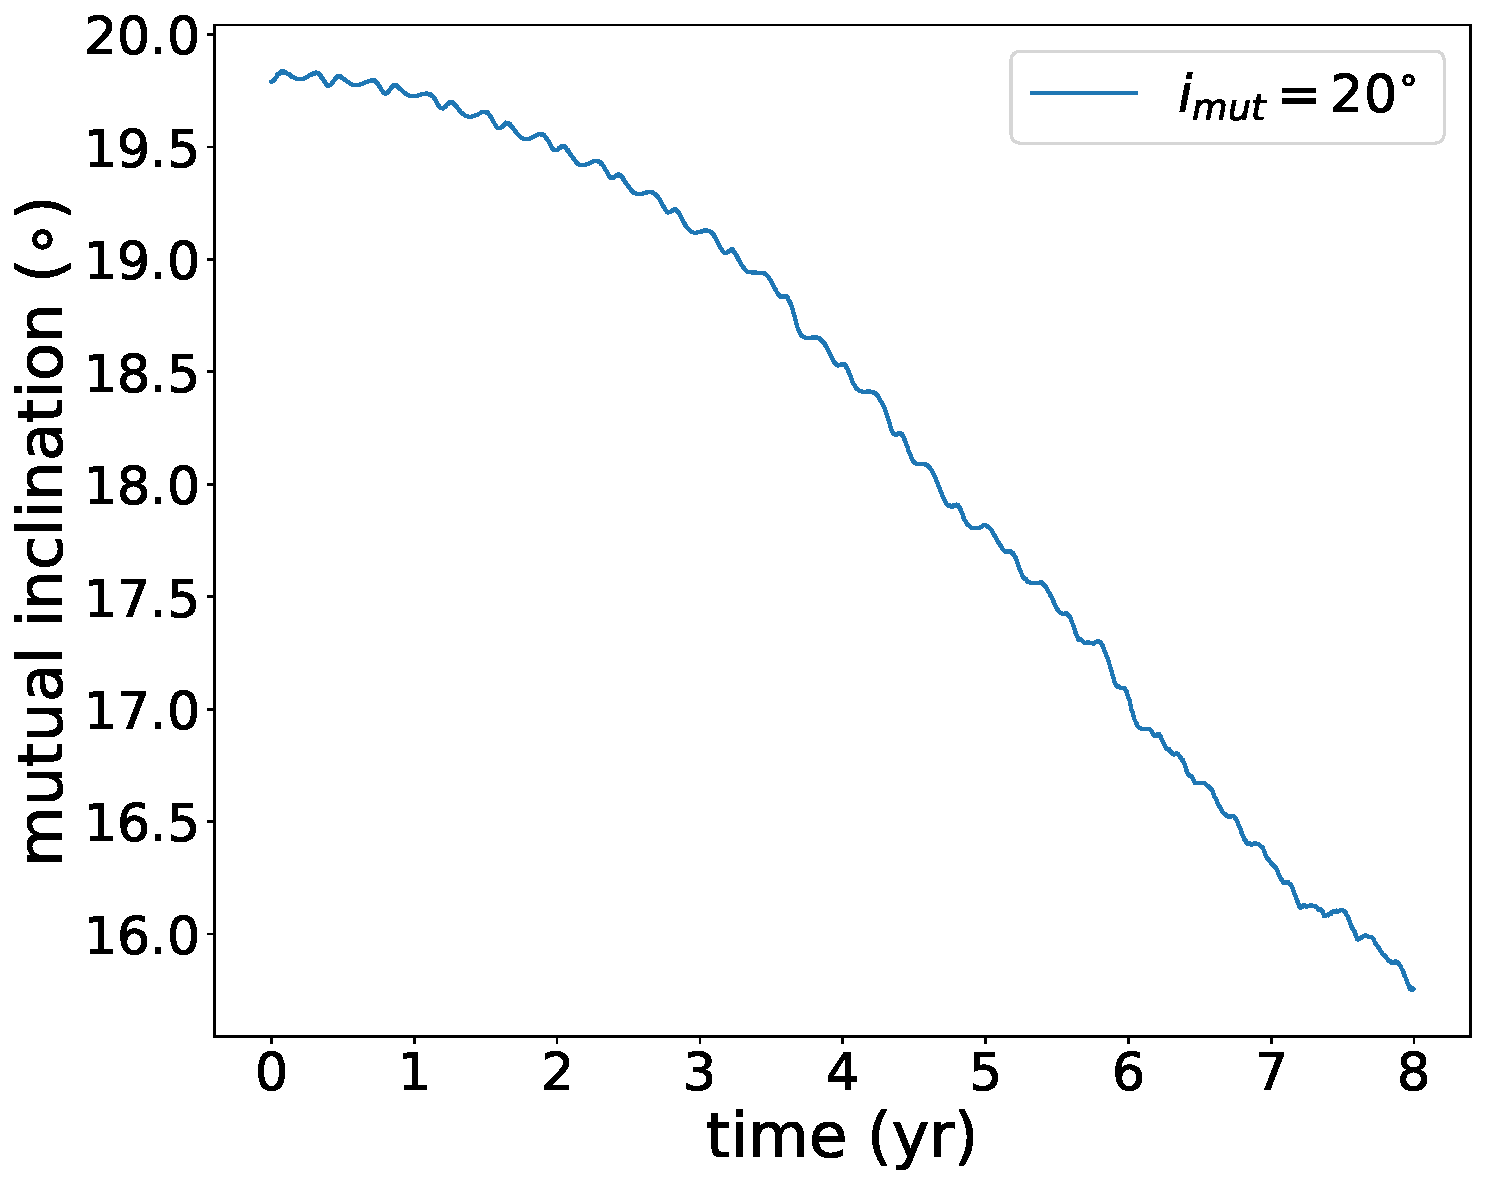
\includegraphics[width=0.9\textwidth]{Thesis/graphs/inclination_case/inc_20.pdf}
    \end{subfigure}%
    \begin{subfigure}{.5\textwidth}
    \centering
    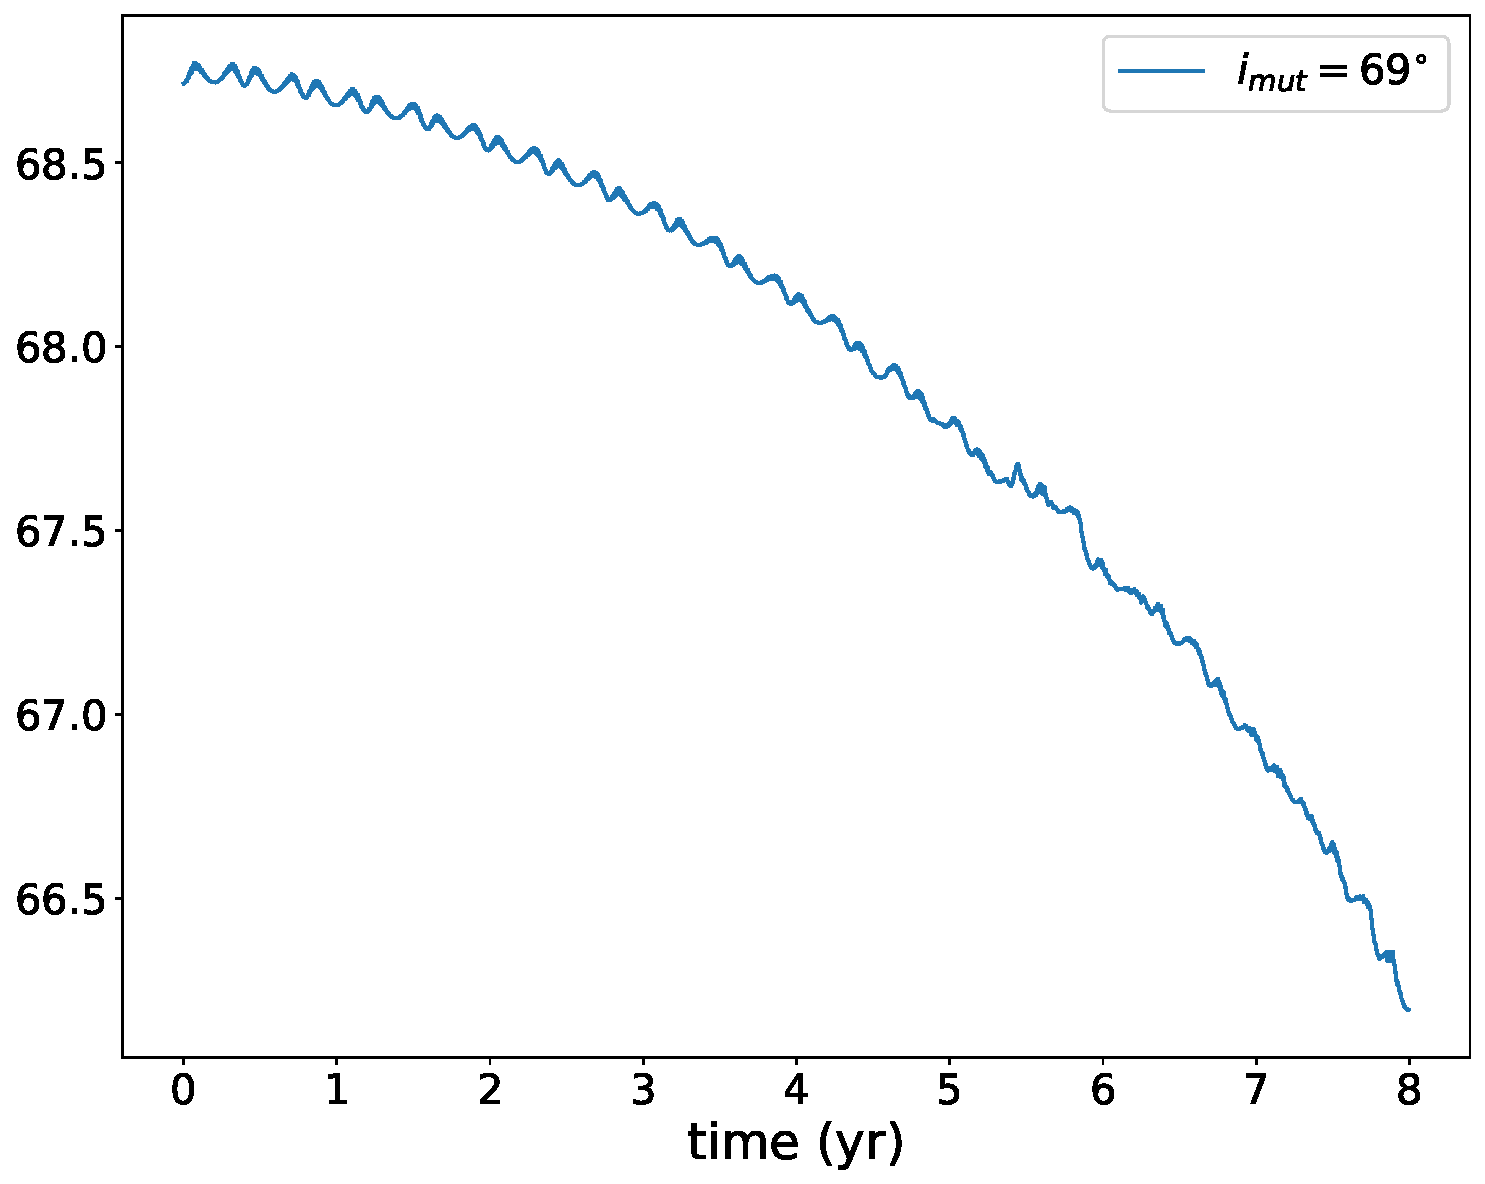
\includegraphics[width=0.9\textwidth]{Thesis/graphs/inclination_case/inc_69.pdf}
    \end{subfigure}
    \caption{ The evolution of the inclination of the outer orbit relative to the inner orbit for initial value: $i_{mut}=20^{\circ}$ (left) and $i_{mut}=69^{\circ}$ (right).}
    \label{fig:mutual_inclination}
\end{figure}

\subsection{Inner orbit}

In \cref{fig:inclination_inner_semimajor_axis} and \cref{fig:inclination_inner_ecc}, I present the evolution of the semi-major axis and eccentricity of the inner orbit for different initial mutual inclinations, respectively. The observed behavior for low inclinations, such as $i_{mut}=0^{\circ}, 20^{\circ}$, has already been described in \cref{sec:accretion}, but the case of $i_{mut}=69^{\circ}$ yields some intriguing results.

Despite underestimating the gas drag, it is evident that I can still extract some valuable insights regarding the evolution of the inner orbit. The inner orbit shrinks with the greatest initial mutual inclination. The reason for this behavior is that the mass stream can successfully cross the inner orbit at high angles, draining orbital angular momentum from the latter. Additionally, because gas drag always tends to shrink the orbit, the observed behavior is qualitatively accurate. The only difference is that including gas drag, the rate of the orbit's decay will be higher or in simple words the observed slope will be steeper. 
\begin{figure}[H]
    \centering
    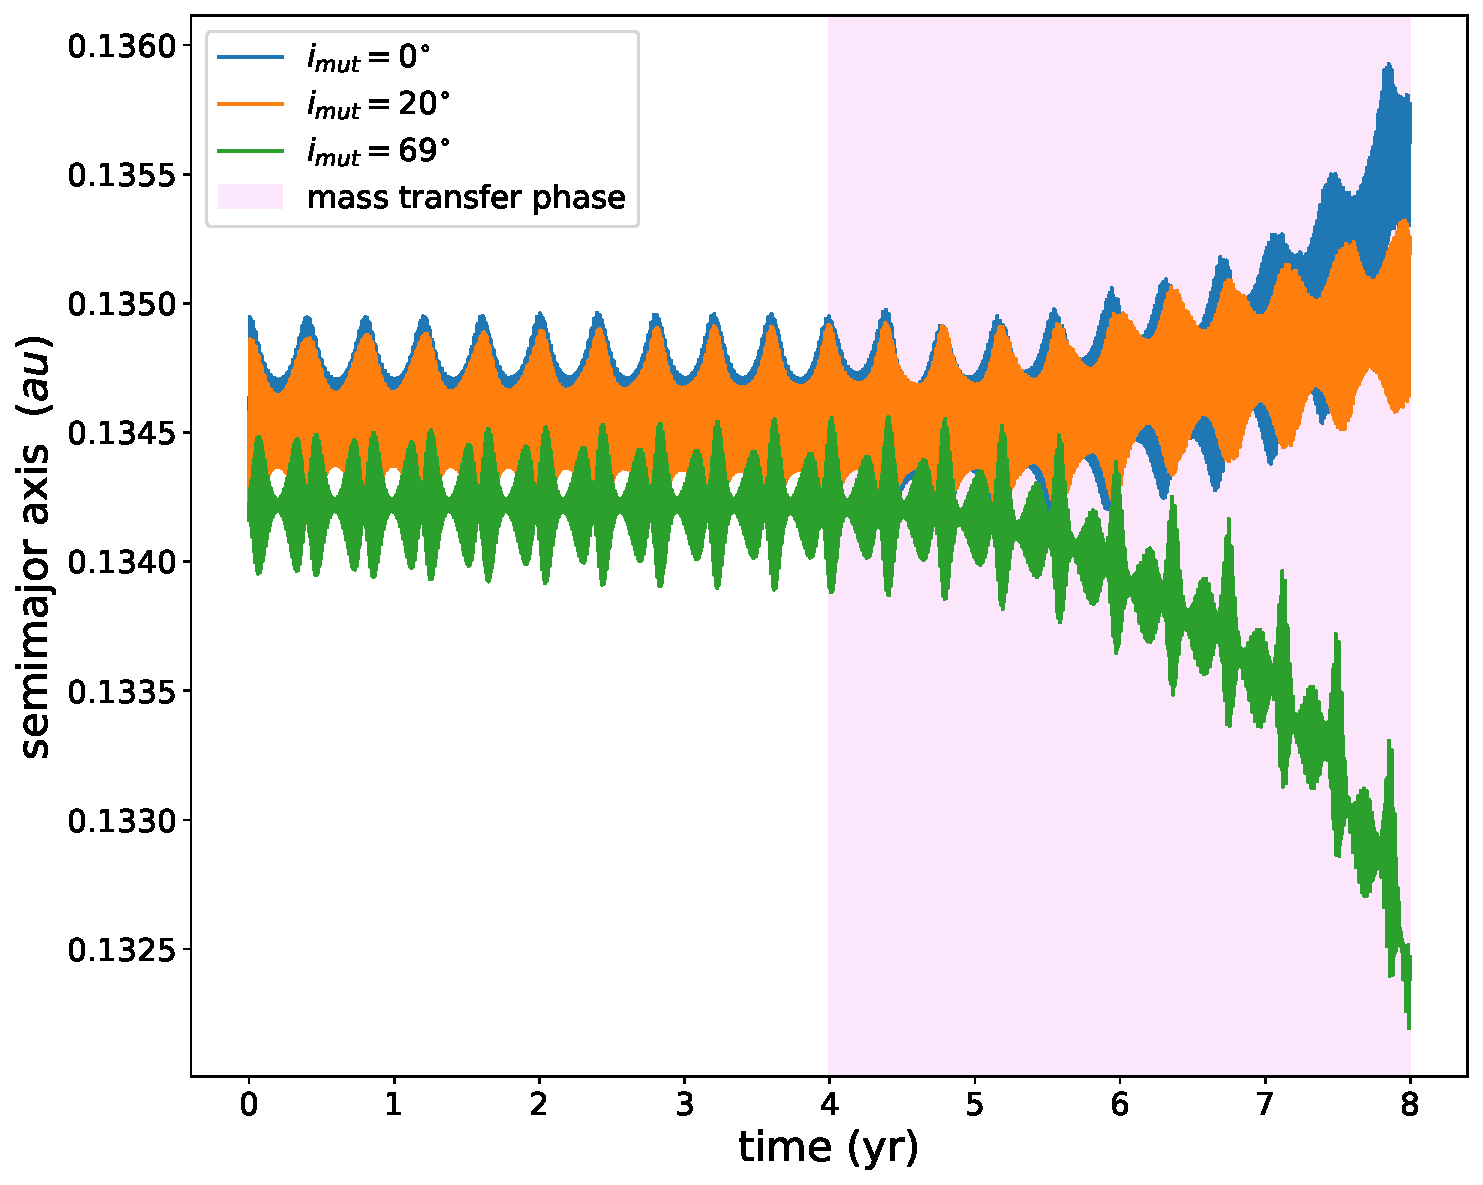
\includegraphics[width=0.9\textwidth]{Thesis/graphs/inclination_case/inclination_inner_semimajor_axis.pdf}
    \caption{Evolution of the semi-major axis of the inner orbit for different initial mutual inclination.}
    \label{fig:inclination_inner_semimajor_axis}
\end{figure}
The $i_{mut}=69^{\circ}$ value was selected intentionally, to test the accuracy of the coupled solver. It is clear, that the latter can resolve Lidov-Kozai cycles. The $i_{mut}=69^{\circ}$ is well inside in the regime where the Lidov-Kozai cycles are expected to occur, see \cref{sub:lidov_kozai}. The eccentricity and mutual inclination are expected to vary periodically. As expected, as the eccentricity increases and the mutual inclination decreases, see \cref{fig:mutual_inclination} and \cref{fig:inclination_inner_semimajor_axis}.
\begin{figure}[!htb]
    \centering
    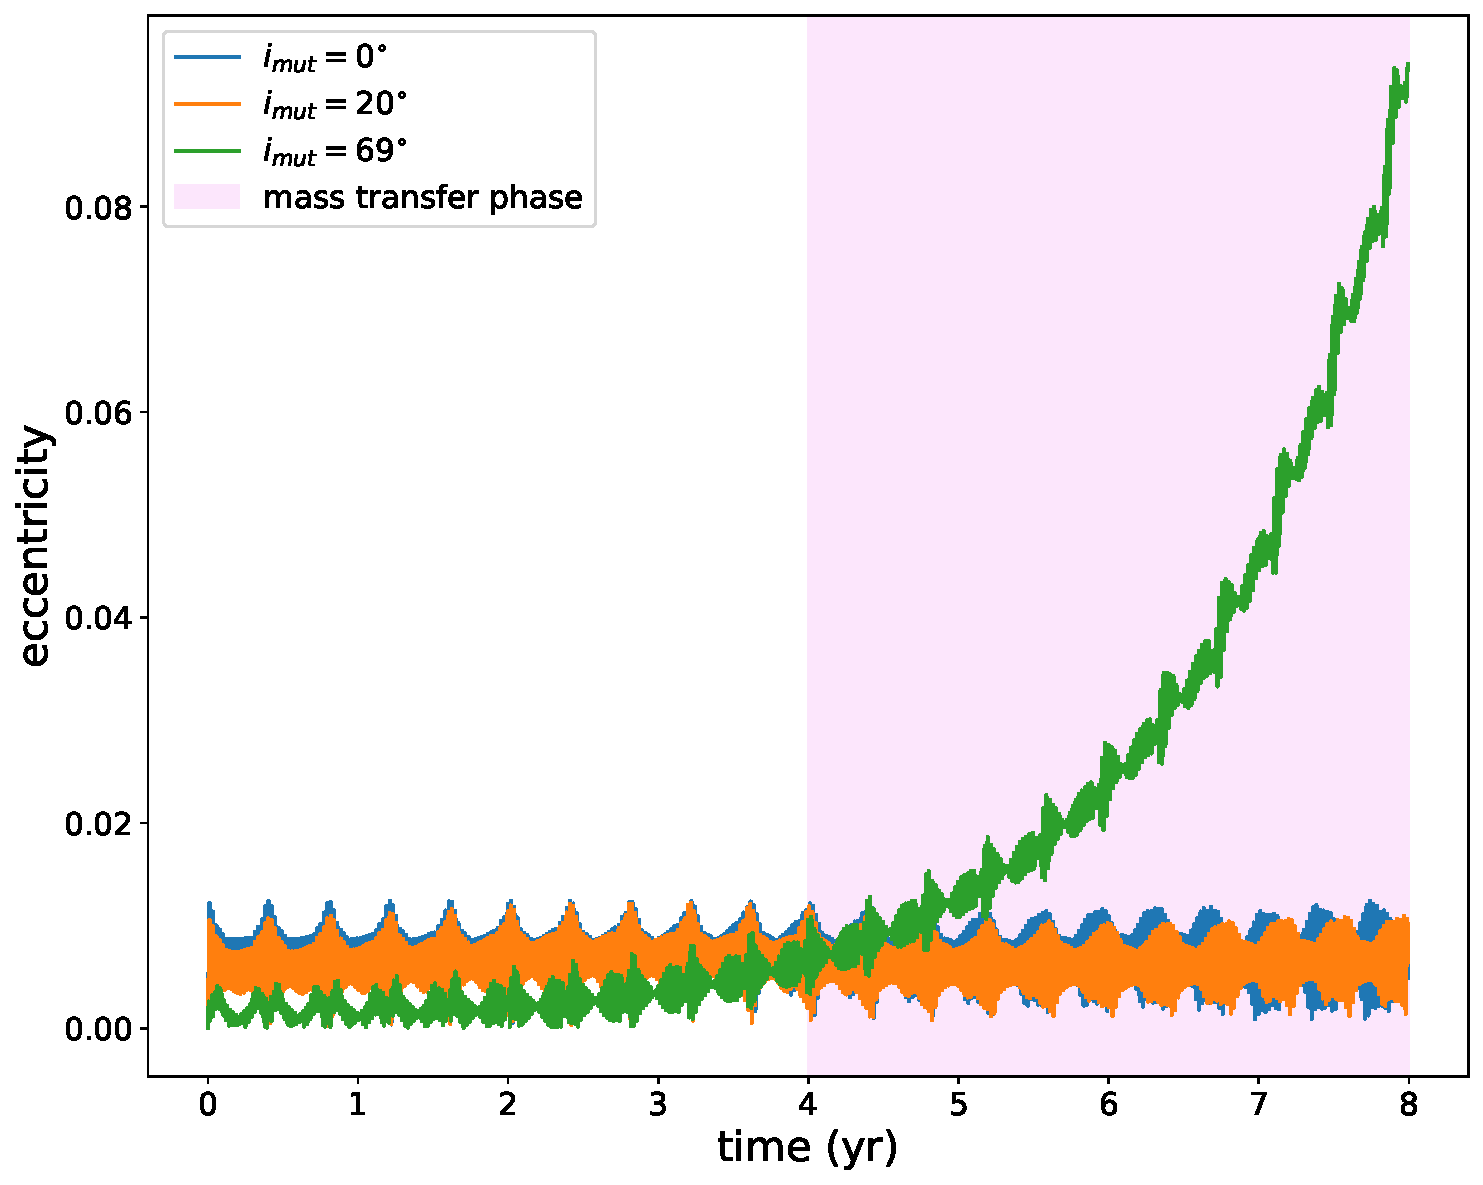
\includegraphics[width=0.9\textwidth]{Thesis/graphs/inclination_case/inclination_inner_ecc.pdf}
    \caption{Evolution of the semi-major axis of the inner orbit for different initial mutual inclination.}
    \label{fig:inclination_inner_ecc}
\end{figure}